\chapter{Evaluation and Analysis}

In previous chapter a few approaches that could improve the genetic solver were presented.
The best results gives a combination of genetic solver with added probabilities and parameter tuning.
Other methods like an adaptive crossover rate or population without duplicated individuals give less effect on the results.

On the other hand, we get valid result only for one problem. What if the problem will be smaller of bigger?
Evaluation was done to find out how all approaches work with different problem sizes. 
\section{Evaluation}
To evaluate genetic solver a benchmark set of 36 problems was used.
Each problem with different characteristics that describes them.

This set was tested with several versions of genetic solver:
\begin{itemize}
	\item basic,
	\item basic with tuned parameters,
	\item with added parameters,
	\item with added parameters and tuning,
	\item with adaptive crossover rate,
	\item with adaptive crossover rate and tuning,
	\item without duplicates in a population,
	\item without duplicates in a population and tuning.
\end{itemize}

Each version of the genetic solver tries 5 times to solve each problem.

Figure~\ref{fig:EvaluationNumberOfSolvedProblems} shows the number of problems in which genetic solver get a valid result.
All previously presented approaches get more valid results in comparison to basic version.
\begin{figure}
	\centering
	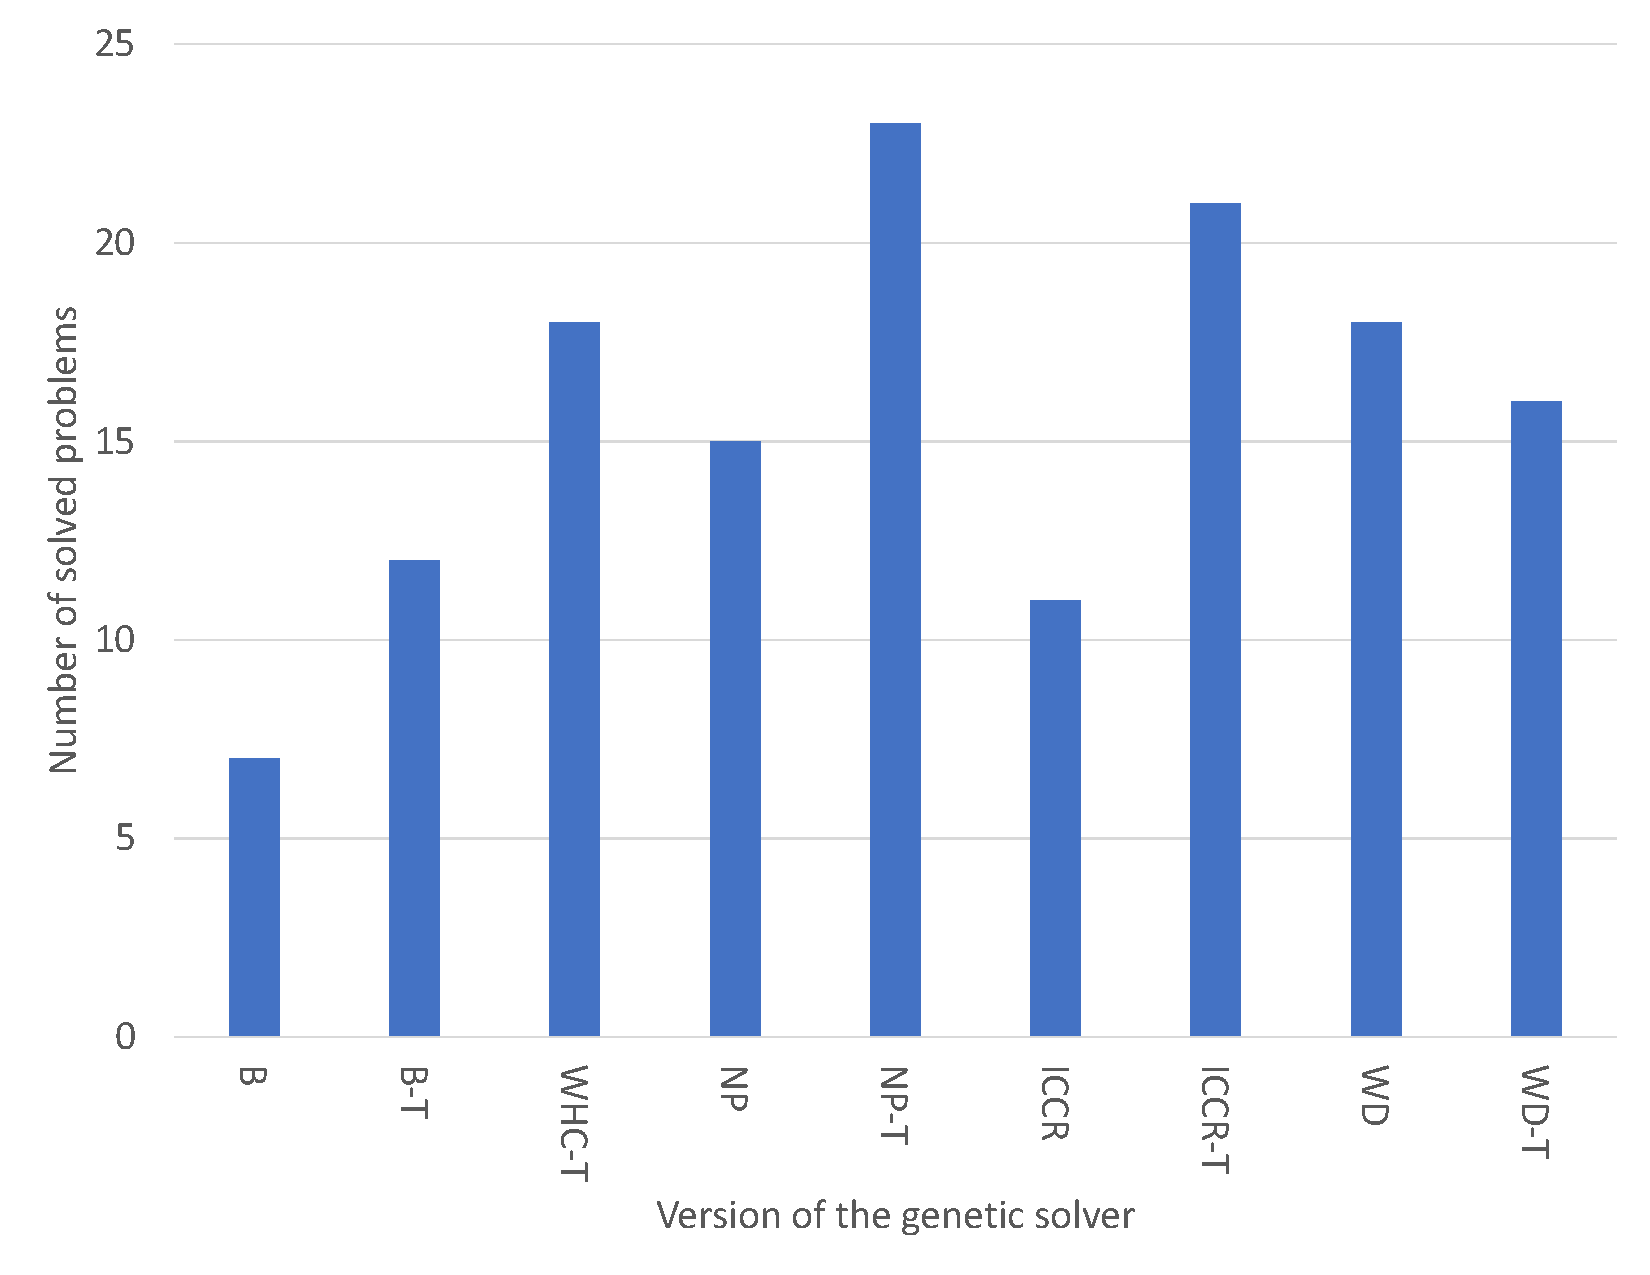
\includegraphics[width=\textwidth]{images/EvaluationNumberOfSolvedProblems.pdf}
	\caption[Number of problems for each version of the genetic solver]{Number of solved problems for each version of the genetic solver}
	\label{fig:EvaluationNumberOfSolvedProblems}
\end{figure}

\todo{when benchmark will be finished I will add more}

But what about energy?


Table~\ref{tab:EnergyTable} shows  the percentage deviation of the found solution from the optimum.
The conclusion from this table is that if solver find out a valid results it will be optimal or near optimal.

\begin{table}
	\begin{tabularx}{\textwidth}{@{}rrrrr@{}}
		\toprule
		\textbf{Problem ID} & \textbf{Basic} &
		\textbf{with new probabilities} & \textbf{without duplicates in population} & \textbf{without duplicates in population + tuning} 
		\tabularnewline
		\midrule
		1 & 1.23 & 0.01 & 0 & 0
		\tabularnewline
		10 & 0.26 & 0.03 & 0 & 0
		\tabularnewline
		13 & 0.05 & 0.05 & 0.15 & 15.0
		\tabularnewline
		19 & 0.19 & 0.19 & 0 & 0
		\tabularnewline
		28 & 0.32 & 0 & 0.02 & 0
		\tabularnewline
		31 & 29.93 & 6.97 & 0.33 & 6.71
		\tabularnewline
		\bottomrule
	\end{tabularx}
	\caption{Table name}\label{tab:EnergyTable}
\end{table}



The results also shows that even with modifications genetic solver could not get valid and optimal results for all problems.


\section{Analysis}
Benchmark showed that genetic solver is not the best choice to solve the MquAT problem.
In this section we presented analysis of results, reasons why described in Chapter~\ref{chapter:Implementation} approaches and 


\begin{itemize}
	\item Good parameter engineering 
	\item Self-adaptive software is not the best thing to optimize!
	\item GA is not the best idea for this kind of problem
\end{itemize}

Plots for analysis:
\begin{itemize}
	\item Search space view
	\item correlation
	\item distribution of two parameters
	\item list for combinations of 3-15
	\item Barplots that shows that solver could find optimal results or near optimal 
	combined chart of validity and objective to parameter
	
\end{itemize}